% Options for packages loaded elsewhere
\PassOptionsToPackage{unicode}{hyperref}
\PassOptionsToPackage{hyphens}{url}
%
\documentclass[final,
  11pt,
]{article}
\usepackage[]{mathpazo}
\usepackage{amsmath}
\usepackage{ifxetex,ifluatex}
\ifnum 0\ifxetex 1\fi\ifluatex 1\fi=0 % if pdftex
  \usepackage[T1]{fontenc}
  \usepackage[utf8]{inputenc}
  \usepackage{textcomp} % provide euro and other symbols
  \usepackage{amssymb}
\else % if luatex or xetex
  \usepackage{unicode-math}
  \defaultfontfeatures{Scale=MatchLowercase}
  \defaultfontfeatures[\rmfamily]{Ligatures=TeX,Scale=1}
\fi
% Use upquote if available, for straight quotes in verbatim environments
\IfFileExists{upquote.sty}{\usepackage{upquote}}{}
\IfFileExists{microtype.sty}{% use microtype if available
  \usepackage[]{microtype}
  \UseMicrotypeSet[protrusion]{basicmath} % disable protrusion for tt fonts
}{}
\makeatletter
\@ifundefined{KOMAClassName}{% if non-KOMA class
  \IfFileExists{parskip.sty}{%
    \usepackage{parskip}
  }{% else
    \setlength{\parindent}{0pt}
    \setlength{\parskip}{6pt plus 2pt minus 1pt}}
}{% if KOMA class
  \KOMAoptions{parskip=half}}
\makeatother
\usepackage{xcolor}
\IfFileExists{xurl.sty}{\usepackage{xurl}}{} % add URL line breaks if available
\IfFileExists{bookmark.sty}{\usepackage{bookmark}}{\usepackage{hyperref}}
\hypersetup{
  pdftitle={Time Series Analysis - STAT 478 - Project},
  pdfauthor={Alexander Towell (atowell@siue.edu)},
  pdfkeywords={time series analysis, known-plaintext attack, encrypted
search, confidentiality measure, estimation},
  hidelinks,
  pdfcreator={LaTeX via pandoc}}
\urlstyle{same} % disable monospaced font for URLs
\usepackage[margin=1in]{geometry}
\usepackage{graphicx}
\makeatletter
\def\maxwidth{\ifdim\Gin@nat@width>\linewidth\linewidth\else\Gin@nat@width\fi}
\def\maxheight{\ifdim\Gin@nat@height>\textheight\textheight\else\Gin@nat@height\fi}
\makeatother
% Scale images if necessary, so that they will not overflow the page
% margins by default, and it is still possible to overwrite the defaults
% using explicit options in \includegraphics[width, height, ...]{}
\setkeys{Gin}{width=\maxwidth,height=\maxheight,keepaspectratio}
% Set default figure placement to htbp
\makeatletter
\def\fps@figure{htbp}
\makeatother
\setlength{\emergencystretch}{3em} % prevent overfull lines
\providecommand{\tightlist}{%
  \setlength{\itemsep}{0pt}\setlength{\parskip}{0pt}}
\setcounter{secnumdepth}{5}
\usepackage{alex}
\ifluatex
  \usepackage{selnolig}  % disable illegal ligatures
\fi

\title{Time series analysis of a confidentiality measure for an Encrypted search system}
\author{Alexander Towell \thanks{\href{mailto:atowell@siue.edu}{\nolinkurl{atowell@siue.edu}}} \\ Southern Illinois University-Edwardsville Math Department}
\date{April 30, 2021}

\begin{document}
\maketitle
\begin{abstract}
We perform a time series analysis of the confidentiality of
an Encrypted search system with respec to a theoretical adversary
who employs a known-plaintext attack on the search agents' Encrypted searches. 
We derive an estimator of the forecast distribution on the confidentiality
measure, which may be used to inform policies such as when and how
frequently a password change may be called for to maintain a minimum
level of confidentiality.
\end{abstract}

{
\setcounter{tocdepth}{3}
\tableofcontents
}
\hypertarget{introduction}{%
\section{Introduction}\label{introduction}}

In \emph{cloud computing}, it is tempting to store confidential data on
(untrusted) cloud storage providers. However, a system administrator may
be able to compromise the confidentiality of the data, threatening to
prevent further adoption of cloud computing and electronic information
retrieval in general.

The primary challenge is a trade-off problem between confidentiality and
usability of the data stored on untrusted systems.
\emph{Encrypted Search} attempts to resolve this trade-off problem.

\begin{definition}
\emph{Encrypted Search} allows authorized search agents to investigate presence
of specific search terms in a confidential target data set, such as a database
of encrypted documents, while the contents, especially the meaning of the target
data set and search terms, are hidden from any unauthorized personnel, including
the system administrators of a cloud server.
\end{definition}

Essentially, \emph{Encrypted Search} enables \emph{oblivous search}. For
instance, a user may search a confidential database stored on an
untrusted remote system without other parties being able to determine
the information need of the user searched (and on more sophisticated
systems, they are also unable to determine which documents were relevant
to the information need).

We denote any untrusted party that has full access to the untrusted
remote system (where the confidential data is stored) the
adversary.\footnote{A system
administrator being a typical example.}

Despite the potential of \emph{Encrypted Search}, \emph{perfect}
confidentiality is not theoretically possible. There are many ways
confidentiality may be compromised. In this paper, we consider an
adversary whose primary objective is to comprehend the confidential
information needs of the search agents by analyzing their history of
\emph{encrypted} queries.

A simple measure of confidentiality is given by the proportion of
queries the adversary is able to comprehend. We consider an adversary
that employs a known-plaintext attack. However, since the
confidentiality is a function of the history of queries, different
histories will result in different levels of confidentiality over time.

We apply time series analysis to estimate the forecast distribution of
the confidentiality measure. The forecast distribution provides the
framework to estimate important security-related questions such as
``what will our mean confidentiality six months from now be?''

We are interested in reasonably medium-term forecasts so that we can
plan accordingly for the future, e.g., determining how frequently
passwords should be reset to try to maintain a base level of
confidentiality. Resetting them too frequently poses an independent set
of problems, both from a security and usability standpoint, but failing
to reset them when the risk of being compromised is too high defeats the
central purpose of Encrypted search.

\hypertarget{encrypted-search-model}{%
\section{Encrypted search model}\label{encrypted-search-model}}

\label{sec:es_model} An information retrieval process begins when a
\emph{search agent} submits a \emph{query} to an information system,
where a query represents an \emph{information need}. In response, the
information system returns a set of relevant objects, such as
\emph{documents}, that satisfy the information need.

An \emph{Encrypted Search} system may support many different kinds of
queries, but we make the following simplifying assumption.

\begin{assumption}
The query model is a \emph{sequence-of-words}.
\end{assumption}

The \emph{adversary} is given by the following definition.

\begin{definition}
The adversary is an untrusted agent that is able to observe the sequence of
queries submitted by authorized search agent.
\end{definition}

The objective of the \emph{Encrypted Search} system is to prevent the
adversary from being able to comprehend the sequence of queries.

\begin{definition}
A \emph{hidden query} represents a confidential \emph{information need} of an
authorized search agent that is suppose to be incomprehensible to the adversary.
\end{definition}

The primary means by which \emph{Encrypted Search} is enabled is by the
use of cryptographic \emph{trapdoors} as given by the following
definition.

\begin{definition}[Trapdoor]
Search agents map \emph{plaintext} search keys to some cryptographic hash,
denoted trapdoors.
\end{definition}

A trapdoor for a \emph{plaintext} search key is necessary to allow an
\emph{untrusted} \emph{Encrypted Search} system to look for the key in a
corresponding confidential data set.

\begin{assumption}
The \emph{Encrypted Search} system uses a simple substitution cipher in which
each search key is mapped to a unique trapdoor signature.
\end{assumption}

The simple substitution cipher is denoted by \begin{equation}
    \operatorname{h} \colon \set{X} \mapsto \set{Y}\,,
\end{equation} where \(\set{X}\) is the set of \emph{plaintext} search
keys and \(\set{Y}\) is the set of \emph{trapdoors}.

Since \(\operatorname{h}\) is one-to-one, it is possible to \emph{undo}
the substitution cipher by some function denoted by \begin{equation}
    \operatorname{g} \colon \set{Y} \mapsto \set{X}
\end{equation} such that \[
    x = \operatorname{g}(\operatorname{h}(x))
\] for every \(x \in \set{X}\).

In a time series, we have \emph{one} entitty and \(T\) measurements of
it over time. A random time series is a sequence of random variables \[
  \{Y_1,Y_2,\ldots,Y_T\},
\] typically denoted by \(\{Y_t\}\) where \(t\) is the time index, which
can continuous or discrete. MoreThe time index is more appro

The measurements are \(d\) dimensional and may be continuous, discrete,
or some mixture. Frequently \(d=1\), which we denote a univariate time
series, and the measurements are continuous.

We use upper-case to denote random variables and lower-case to denote
realizations, thus \(Y_t\) is a random value and \(y_t\) is the
realization of \(Y_t\).

Thus, a realization of the time series \(\{Y_t\}\) is given by denoted
by \(\{y_t\}\).

The time series of \emph{plaintext} keyword searches submitted by the
search agents is denoted by \(\{x_t\}\). It is a \(d=1\) dimensional
time series with a discrete time index and a discrete response.

The adversary may may directly observe \(\{x_t\}\). Instead, he observes
a time series of ciphers.

\begin{definition}
The \emph{cipher} $\{c_t\}$ is a discrete time and discrete
response time series defined as
$$
  c_t = \operatorname{h}(x_t).
$$
\end{definition}

Since the time series of \emph{plaintext} is a priori non-deterministic,
we model it as a random time series \(\{X_t\}\) such that
\begin{equation}
    \Pr(X_j = x_j | X_1 = x_1,\ldots,X_{j-1} = x_{j-1}).
\end{equation} That is to say, our plaintext language model does not
incorporate other kinds of information, such as who the search agent is
or what time of day it is. In section \ref{sec:future}, we consider
extensiosn of the model.

Since \(\{c_t\}\) is a function of \(\{x_t\}\), we may model the ciphers
as a random time series \(\{ C_t \}\) where
\(C_j = \operatorname{h}(X_j)\).

\hypertarget{threat-model-known-plaintext-attack}{%
\section{Threat model: known-plaintext
attack}\label{threat-model-known-plaintext-attack}}

\label{sec:threat} The primary source of information is given by the
observable time series of ciphers \(\{c_t\}\), which is induced by the
unobserved time series of plaintext \(\{x_t\}\).

Other potential sources of information, such as side-channel
information, is not included in the model we consider in this paper. See
section \ref{sec:future} for some preliminary thoughts on this expanded
topic.

In the threat model described in section \ref{sec:threat}, the adversary
is interested in estimating \(\{x_t\}\). However, the adversary is only
able to observe \(\{c_t\}\). Thus, the adversary's objective is to infer
the plaintext from the ciphers using frequency analysis attacks, in
particular a \emph{known-plaintext} attack.

In a known-plaintext attack, the objective of the adversary is to learn
how to \emph{undo} the substitution cipher \(\operatorname{h}\) with
\(\operatorname{g}\).

\begin{assumption}
The inverse substitition cipher $\operatorname{g}$ is not known to the adversary.
\end{assumption}

A maximum likelihood estimator of \(\operatorname{g}\) is given by \[
    \hat{\operatorname{g}} = \argmax_{\operatorname{g} \in G}
    \Pr(X_1 = \operatorname{g}(c_1)) \prod_{t=2}^{T} \Pr(X_t =
    \operatorname{g}(c_t) | X_{t-1} = \operatorname{g}(c_{t-1}),
            \ldots, X_1 = \operatorname{g}(c_1))
\] where \(G\) is the set of all possible mapping functions from ciphers
\(\set{Y}\) to plaintexts \(\set{X}\).

If two plaintexts \(x,x' \in \set{X}, x \neq x'\), may be exchanged
without changing the probability of \(\{x_t\}\), then they are
\emph{indistinguishable} and \(\hat{\operatorname{g}}\) is
\emph{inconsistent}. However, the adversary does not need to be perfect
for the confidentiality measure to be compromised. If some of the
plaintexts are inexchangeable, then the adversary may learn
\emph{something} about \(\{x_t\}\) by observing \(\{c_t\}\).

The greater the uniformity of \(\{X_t\}\) the greater the variance of
\(\hat{\operatorname{g}}\). At the limit of maximum uniformity, where
every pair of plaintext is exchangeable, the adversary can learn nothing
about \(\{x_t\}\) by observing \(\{c_t\}\). Natural languages have a
high degree of non-uniformity and so the primary concern of the
adversary is the divergence between the \emph{true} distribution and the
\emph{known-plaintext} distribution.

\begin{assumption}
The adversary knows some approximation of $\{X_t\}$.
\end{assumption}

The \emph{known-plaintext} distribution may be used to solve an
approximation of the MLE \(\hat{\operatorname{g}}\).

\begin{definition}
In a \emph{known-plaintext attack}, the adversary substitutes the unknown true
distribution with the known-plaintext distribution and solves the MLE under
this substituted distribution.
\end{definition}

\section{Confidentiality measure}

We are interested in measuring the degree of confidentiality as given by
the following definition.

\begin{definition}
Given a time series $\{c_{t'}\}$, the confidentiality measure is a time series
$\{\pi_t\}$ defined as the fraction of ciphers in $\{c_{t'}\}$ that the adversary
successfully maps to \emph{plaintext} where $t' = N t$.
That is,
\begin{equation}
\label{eq:accuracy}
    \pi_t = \frac{\delta_t}{N t}\,,
\end{equation}
where
\begin{equation}
    \delta_t = \sum_{t'=1}^{N t} [\operatorname{g}(c_{t'}) = \hat{\operatorname{g}}(c_{t'})]\,.
\end{equation}
\end{definition}

Note that \(N\) denotes the fact that we take one measurement of the
confidentiality every time a multiple of \(N\) ciphers are observed.

The measure \(\pi_t\) can be understood as the marginal probability that
the adversary is able to decode an incoming cipher to plaintext at
around time \(t\). However, far more revealingly, the adversary may go
back through the history of ciphers and decode proportion \(\pi_t\) to
plaintext.

If we specify that \(\pi^*\) is the minimum confidentiality measure we
wish to maintain, then it is essential that we stop generating
\(\{c_t\}\) at or before time \(T^*\) where \[
  T^* = \argmin_{T} \pi_T > \pi^*.
\] That is, we stop generating \(\{c_{t'}\}\) before the amount of
information in it is sufficient for the adversary to decode more than
proportion \(\pi^*\) of the data. We do not need to stop Encrypted
search queries at time \(T^*\), we only need to change the cipher, i.e.,
substitute the mapping function \(\operatorname{h}\) that maps
plaintexts to ciphers with some other mapping function, which is
typically done by requiring users to change passwords periodically. This
is where \emph{forecasting} \(\{\pi_t\}\) plays a central role.

\hypertarget{forecasting-model}{%
\subsection{Forecasting model}\label{forecasting-model}}

As a function of a \emph{random time series} \(\{C_{t'}\}\), we may
model \(\pi_t\) as being generated by the random time series
\(\{\Pi_t\}\). If \(\pi_{t}\) is not known, i.e., \(\Pi_{t}\) has not
been observed, then \(\Pi_{t}\) is a probability distribution on the
measure at time \(t\). If \(\pi_{1},\pi_{2},\ldots,\pi_{T}\) is given,
then \(\Pi_{T+h|T}\) is a \emph{conditional}
distribution\footnote{$\Pi_{T+h}$ given $\Pi_1 = \pi_1,\ldots,\Pi_T = \pi_T$.}
known as the \(h\)-step forecast distribution at time \(T\) whose
expectation is denoted by \(\pi_{T+h|T}\).

Our primary interest is in \emph{forecasting} an observed time series
\(\{\pi_t\}\), e.g., if we observe \(\{\pi_1,\pi_2,\ldots,\pi_T\}\), we
wish to estimate the mean of the \(h\)-step forecast \(\pi_{T+h|T}\).
Since \(\pi_{T+h|T}\) is not known, we seek an estimator
\(\hat{\pi}_{T+h|T}\).

\hypertarget{data-description}{%
\section{Data description}\label{data-description}}

The \emph{accuracy} \(\{\pi_t\}\) of the adversary is the single entity
we are observing and we have \(T\) measurements of it over logical time.

The confidentiality data \(\{\pi_t\}\) depends upon two other time
series, the plaintext (keyword searches) \(\{x_t\}\) and the ciphers
\(\{c_t\}\), which Alex Towell generated in 2016 using the following
steps:

\begin{enumerate}
\item The parameters of a Bigram language model were estimated from a large
corpus of plaintext.
(The source of the particular corpus used has been lost.)
\item The estimated Bigram language model was conditionally sampled from to
generate plaintexts $\{x_t\}$.
\item Each plaintext $x_t$ was cryptographically hashed to a cipher
$c_t = \operatorname{h}(x)$ to generate ciphers $\{c_t\}$.
\end{enumerate}

Note that \(\{x_t\}\) and \(\{c_t\}\) are not the primary time series of
interest in our analysis. Rather, our primary interest is in the
confidentiality measures \(\{\pi_t\}\). To generate this time series,
the following steps were taken:

\begin{enumerate}
\item The function $\operatorname{g}$ that maps ciphers to plaintext is
estimated after every $N=50$ observations of the cipher time series using a
MLE under a unigram language model (some information in the bigram model is not
being used by the estimator, which reduces its efficiency) on a different corpus
judged to be similiar to the one used to generate $\{x_t\}$.
Thus, the unigram MLE of $\operatorname{g}$ at time $T$ is given by
$$
    \hat{\operatorname{g}}_T = \argmax_{\operatorname{g} \in G}
    \prod_{t=1}^{T} \hat{\Pr}(X_t = \operatorname{g}(c_t)).
$$

Note that $\hat{\operatorname{g}}_T$ is inconsistent since it does not converge
in probability to $\operatorname{g}$ as a consequence of the adversary's
estimation of $\Pr(X_t)$ with $\hat{\Pr}(X_t)$.

This inconsistency was motivated out of a desire to be more realistic, since an
adversary who is performing the known-plaintext attack cannot in practice know
the underlying distribution of $\{x_t\}$ used to generate the keyword searches.
\item The confidentiality measure at time $t$, denoted by $\pi_t$, is computed
using $\hat{\operatorname{g}}_{t}$.
\end{enumerate}

\hypertarget{time-series-analysis-of-pi_t}{%
\section{\texorpdfstring{Time series analysis of
\(\{\pi_t\}\)}{Time series analysis of \textbackslash\{\textbackslash pi\_t\textbackslash\}}}\label{time-series-analysis-of-pi_t}}

It seems clear that the adversary's accuracy at a particular time will
be correlated with lagged (previous) values of its accuracy and the
closer in time they are the more heavily correlated they will generally
be (barring exceptions like seasonality).

We partition the data into a training set and a test set. We will not
look at the test set until later when we evaluate the model. Here is a
quick glimpse of the training set data:

\begin{verbatim}
## [1] 0.358159 0.351208 0.347271 0.346403 0.352666 0.350445
\end{verbatim}

\hypertarget{visualization-and-stationary-transformations}{%
\subsection{Visualization and stationary
transformations}\label{visualization-and-stationary-transformations}}

If the time series data can be transformed to meet the stationary
conditions, then the ARIMA model for the (correlated) residuals is
generally a reasonable choice. A stationary time series is given by:

\begin{enumerate}
\item The mean is not a function of time.
\item The variance is constant.
\item The autocorrelation is a function of lag rather than time.
\end{enumerate}

A plot of the training partition of \(\{\pi_t\}\) is shown in
figure \ref{fig:fa}.

\begin{figure}
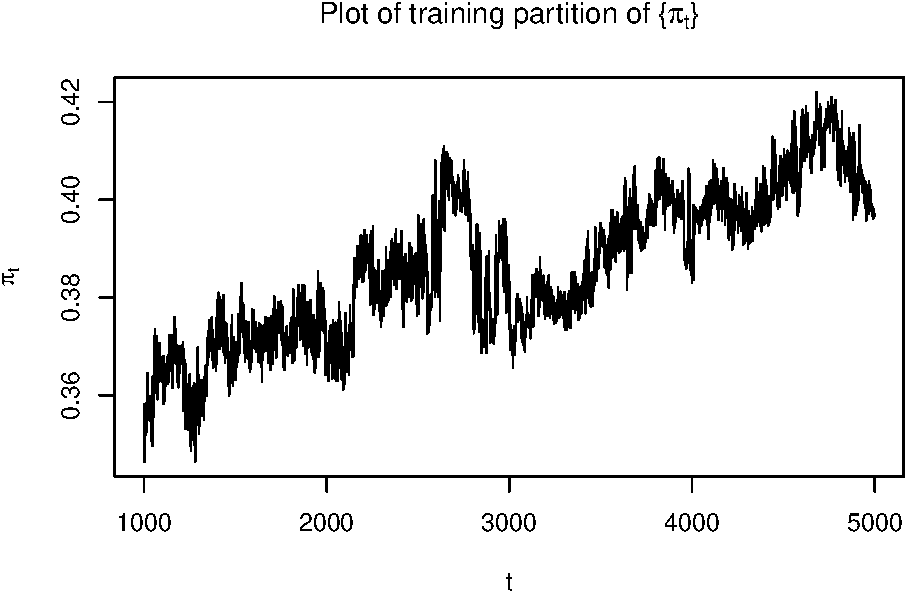
\includegraphics{paper_files/figure-latex/unnamed-chunk-2-1.pdf}
\caption{A non-stationary time series plot.}
\label{fig:fa}
\end{figure}

It appears non-stationary.
A plot of the sample ACF and PACF are shown in figure \ref{fig:f0}.

\begin{figure}
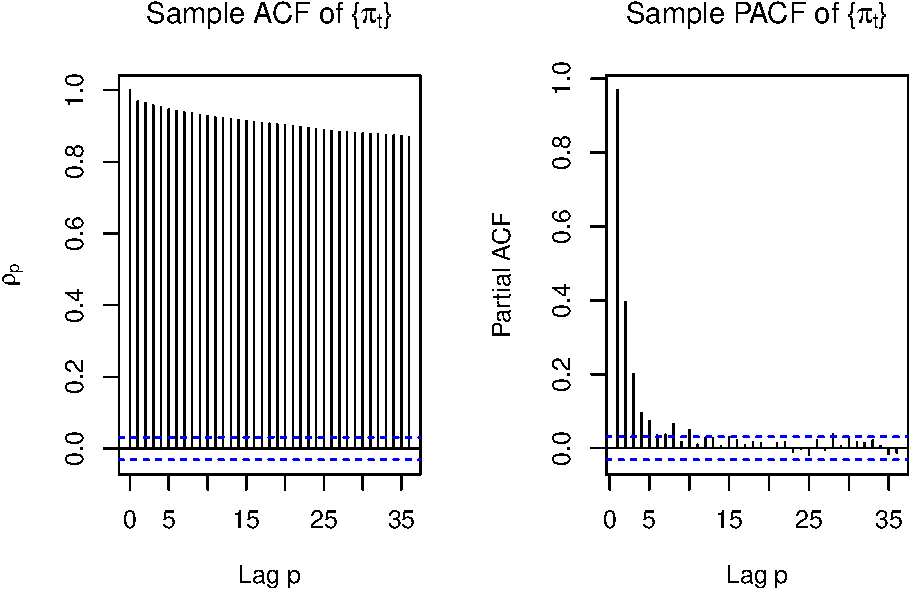
\includegraphics{paper_files/figure-latex/unnamed-chunk-3-1.pdf}
\caption{Highly correlated sample ACF and PACF.}
\label{fig:f0}
\end{figure}

We see that the ACF indicates that \(\{\pi_t\}\) has significant
autocorrelation. While this is clearly non-stationary, the variance
seems constant and thus a transformation to make the variance more
uniform, such as a log-transformation, seems unnecessary.

Since there is not necessarily an obvious pattern in the data, we will
avoid the use of procedures like fitting a regression model (for
detrending) and instead try some order of differencing. Differencing is
a non-parametric approach that can often transform a non-stationary time
series into a stationary one, where the \(d\)-th difference of
\(\{\pi_t\}\) is denoted by \(\nabla^d\{\pi_t\}\). Moreover, since it is
non-parametric, differencing has the added benefit of being able to
dynamically respond to changes in the data, unlike with regression which
treats the trend as deterministic.

\begin{figure}
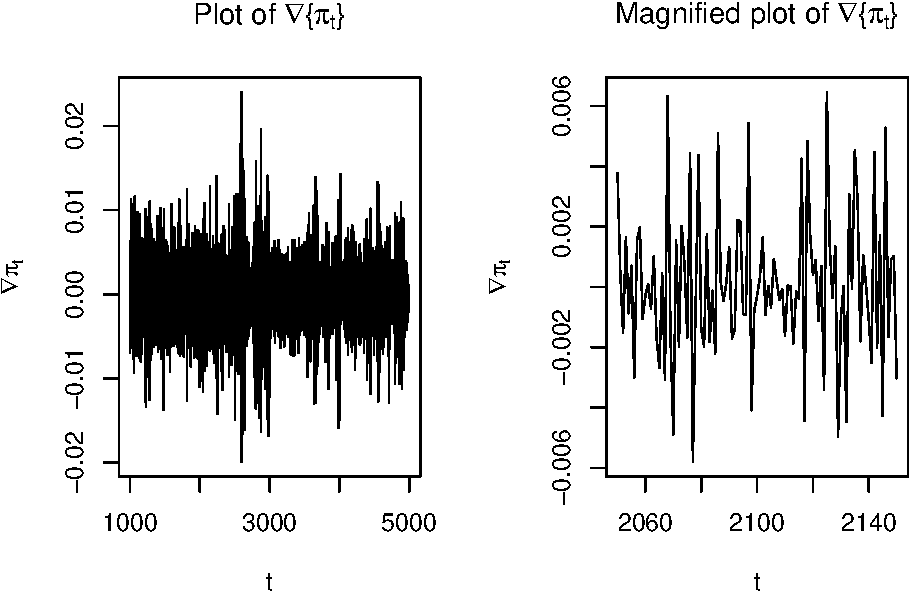
\includegraphics{paper_files/figure-latex/unnamed-chunk-4-1.pdf}
\caption{Time plots of $\nabla \{\pi_t\}$.}
\label{fig:f1}
\end{figure}

In figure \ref{fig:f1}, we plot the differenced process \(\nabla\{\pi_t\}\).
We see that the trend has been removed, the values are centered around
zero, and the variance is constant. We believe this may be stationary.
We perform the augmented Dickey-Fuller
test\cite{noauthor_dickeyfuller_2021} as a more objective measure.

\begin{verbatim}
## Augmented Dickey-Fuller Test
## Dickey-Fuller = -20.37, Lag order = 15, p-value = 0.01
## alternative hypothesis: stationary
\end{verbatim}

The \(p\)-value of the Dickey-Fuller hypothesis test is less than
\(0.01\), which we consider to be very strong evidence against the null
hypothesis of non-stationary data. Bolstered by this test, we proceed
with trying to find an ARIMA model for the residuals.

\hypertarget{arima-model-selection}{%
\subsection{ARIMA model selection}\label{arima-model-selection}}

There are perhaps three primary reasons we would want to infer a general
model for \(\{\pi_t\}\): prescription, description, and in our case,
\emph{prediction}.

Guided by the principle of \emph{parsimony}, we have a bias for simpler
models, i.e., Occam's razor. As justification for this bias, consider
the following. Assume there is some unknown process \(M\) that generated
data \(\{\pi_t\}\). If we have parametric model \(M'\) with many degrees
of freedom (dimension of parameter space), we may find parameters for it
that fit it to \(\{\pi_t\}\) with a very small sum of squared residuals.

However, if \(M'\) is unnecessarily complex, it is unlikely to
\emph{generalize} very well, i.e., on new data \(M\) and \(M'\) may
diverge significantly. In this case, we say that \(M'\) is overfitted to
the observed data \(\{\pi_t\}\). Of course, if a simpler model cannot
even sufficiently model the observed data \(\{\pi_t\}\), it is hard to
justify as an approximation of \(M\). Thus, we have a variance-bias
trade-off\cite{bias_variance}.

Since ARIMA models are parameterized by \(p\), \(d\), and \(q\), which
respectively specify the order of the autoregression component, the
order of the difference, and the order of the moving average component,
we have a bias for ARIMA models with relatively small \(p\), \(d\), and
\(q\). Note that there are many heuristics that model this bias, such as
the Akaike information criterion (AIC), but we will decide upon a subset
of candidate models that leans heavily on a more hands-on analysis.

A plot of sample ACF and PACF of the differenced time series $\nabla \{\pi_t\}$
is shown in figure \ref{fig:f3}.

\begin{figure}
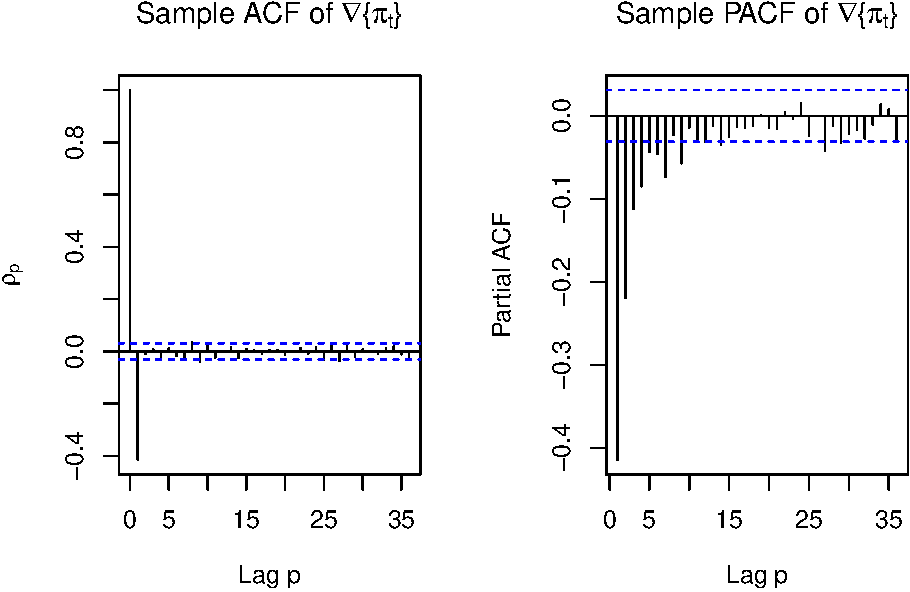
\includegraphics{paper_files/figure-latex/unnamed-chunk-6-1.pdf}
\caption{Sample ACF and PACF of $\nabla \{\pi_t\}$, which appear far more stationary.}
\label{fig:f3}
\end{figure}


Since the ACF cuts off after lag \(1\) and the PACF decays
exponentially, we speculate that \(\nabla\{\pi_t\}\) may be an MA(1)
process. We use the EACF plot to try to help determine other possible
orders of the ARIMA model:

\begin{verbatim}
## AR/MA
##   0 1 2 3 4 5 6 7 8 9 10 11 12 13
## 0 x o o o o o o x x x o  o  o  o 
## 1 x x o o o o x o o o o  o  o  o 
## 2 x x x o o o x o o o o  o  o  o 
## 3 x x x x o o o o o o o  o  o  o 
## 4 x x x x x o o o o o o  o  o  o 
## 5 x x x x x x o o o o o  o  o  o 
## 6 x x x x x o x o o o o  o  o  o 
## 7 x x x x x x x o o o o  o  o  o
\end{verbatim}

Ignoring the set small set of \(x\)'s above the main diagonal of zeros,
we see that \(\{\nabla \pi_t\}\) seems to be compatible with
\(\arma(0,1)\),\(\arma(0,2)\), and \(\arma(1,2)\). We will analyze these
three.

\hypertarget{model-construction-and-evaluation}{%
\subsection{Model construction and
evaluation}\label{model-construction-and-evaluation}}

A good model will yield residuals \(\{e_t\}\) that look like zero mean
white noise:
\begin{enumerate}
\item They are are uncorrelated.
If there are correlations, the residuals contain information that may be used to
estimate a better model.
\item They have zero mean.
If they  have a non-zero mean, then the model (and forecasts) are biased.
\item They have constant variance.
\end{enumerate}

\hypertarget{ima11}{%
\subsubsection{IMA(1,1)}\label{ima11}}

This is the simplest model of the three, and the simplest ARIMA model
that seemed compatible with the data. When we fit the \(\arima(0,1,1)\)
model to the time series data, we get the following result.

\begin{verbatim}
##        ma1 
## -0.5705635
\end{verbatim}

To assess whether the model results in uncorrelated residuals, we
inspect figure \ref{fig:resv}.

\begin{figure}
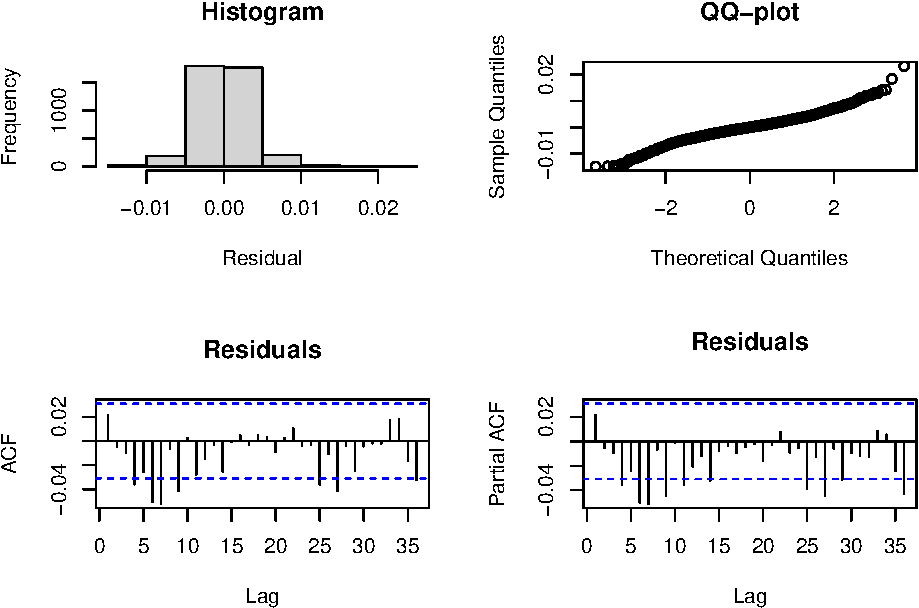
\includegraphics{paper_files/figure-latex/unnamed-chunk-9-1.pdf}
\caption{Plots to conduct stationary assessments of $\arma(1,1)$.}
\label{fig:resv}
\end{figure}

The histogram looks symmetric about \(0\) but the Q-Q suggests a lack of
normality in the residuals. More telling, plots of the sample ACF and
PACF of the residuals are evidence of high correlation. We reject this
model.

\hypertarget{ima12}{%
\subsubsection{IMA(1,2)}\label{ima12}}

When we fit \(\arima(0,1,2)\) to the time series data, we get the
following results.

\begin{verbatim}
##         ma1         ma2 
## -0.55254743 -0.04124893
\end{verbatim}

To assess whether the model results in uncorrelated residuals, we
inspect the plots in figure \ref{fig:res3}.

\begin{figure}
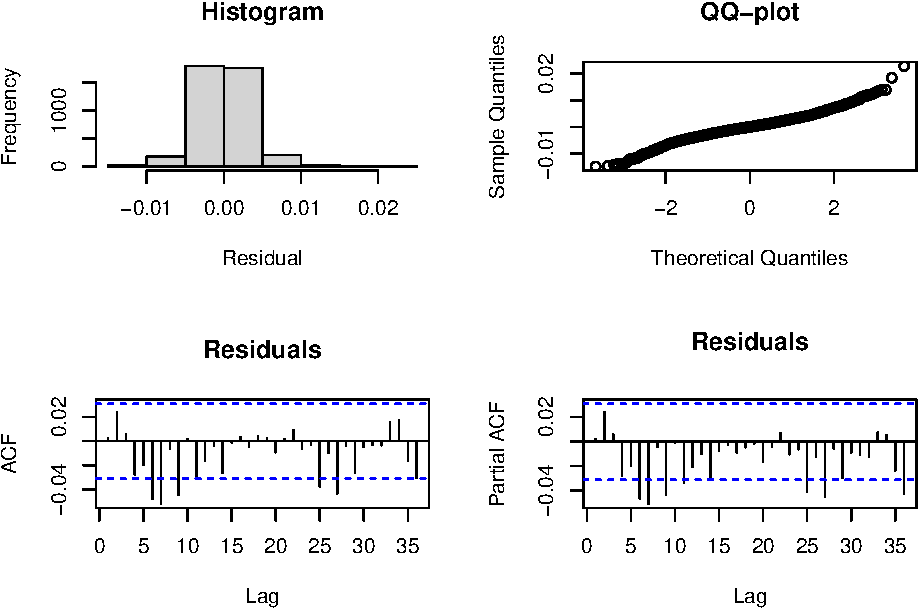
\includegraphics{paper_files/figure-latex/unnamed-chunk-11-1.pdf}
    \caption{Plots to conduct stationary assessments for $\arma(0,1,2)$.}
    \label{fig:res3}
\end{figure}

The histogram looks symmetric about \(0\) but, again, the Q-Q suggests a
lack of normality in the residuals. Note that this is not strictly
required. More telling, plots of the sample ACF and PACF of the
residuals are evidence of high correlation. We reject this model.

\hypertarget{arima112}{%
\subsubsection{ARIMA(1,1,2)}\label{arima112}}

When we fit the \(\arima(1,1,2)\) model to the time series data, we get
the following results.

\begin{verbatim}
##        ar1        ma1        ma2 
##  0.8839643 -1.4423574  0.4689439
\end{verbatim}

To assess whether the model results in uncorrelated residuals, we
inspect figure \ref{fig:res1}.

\begin{figure}
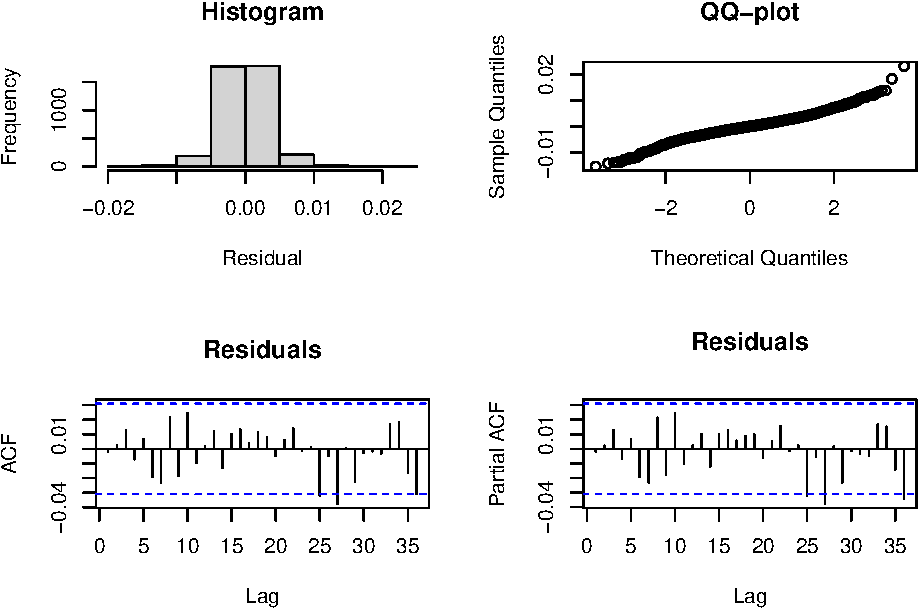
\includegraphics{paper_files/figure-latex/unnamed-chunk-13-1.pdf}
\caption{Plots to conduct stationary assessments of $\arma(1,1,2)$.}
\label{fig:res1}
\end{figure}

The histogram looks symmetric about \(0\) but, again, the Q-Q suggests a
lack of normality in the residuals. However, the sample ACF and PACF
seem reasonable. We perform the Ljung-Box hypothesis (lag = 10) test on
the residuals of the model for a more objective measure of white noise.

\begin{verbatim}
## Box-Ljung test
## data: model.3$residuals
## X-squared = 10.333, df = 7, p-value = 0.1705
\end{verbatim}

The null hypothesis is that the residuals for the model are white noise.
The test reports a \(p\)-value of \(0.171\), which we consider to be
strong evidence in support of the white noise hypothesis.

We choose this model. Since only one model seemed like a reasonable fit,
measures like AIC were not needed.

What follows ia a summary of the chosen model.

\begin{verbatim}
## ARIMA(1,1,2) 
## 
## Coefficients:
##          ar1      ma1     ma2
##       0.8840  -1.4424  0.4689
## s.e.  0.0276   0.0338  0.0266
## 
## sigma^2 estimated as 1.088e-05:  log likelihood=17177.64
## AIC=-34347.27   AICc=-34347.26   BIC=-34322.1
\end{verbatim}

We present it in the more familiar form given by \[
  (1 - 0.884 \backshift) \nabla Y_t = (1 + 1.442 \backshift - 0.469 \backshift^2) e_t
\] or, equivalently, \[
  (1 - 0.884 \backshift) \nabla Y_t = (1 - 0.273 \backshift) (1 + 1.715 \backshift) e_t
\] where \(\{e_t\}\) is given by zero mean white noise, \[
  e_t \sim \operatorname{WN}(\mu=0,\sigma=0.0033).
\]

\hypertarget{forecasting}{%
\subsection{Forecasting}\label{forecasting}}

One of the primary goals of this time series analysis is forecasting, or
predicting, the future accuracy of the adversary, i.e.,
\(\hat{\pi}_{T+h|T}\).
At \(T=5000\), we perform a forecast up to
\(h=1000\) steps ahead, \(\hat{\pi}_{T+h|T}\).
See figure \ref{fig:forecast}.

\begin{figure}
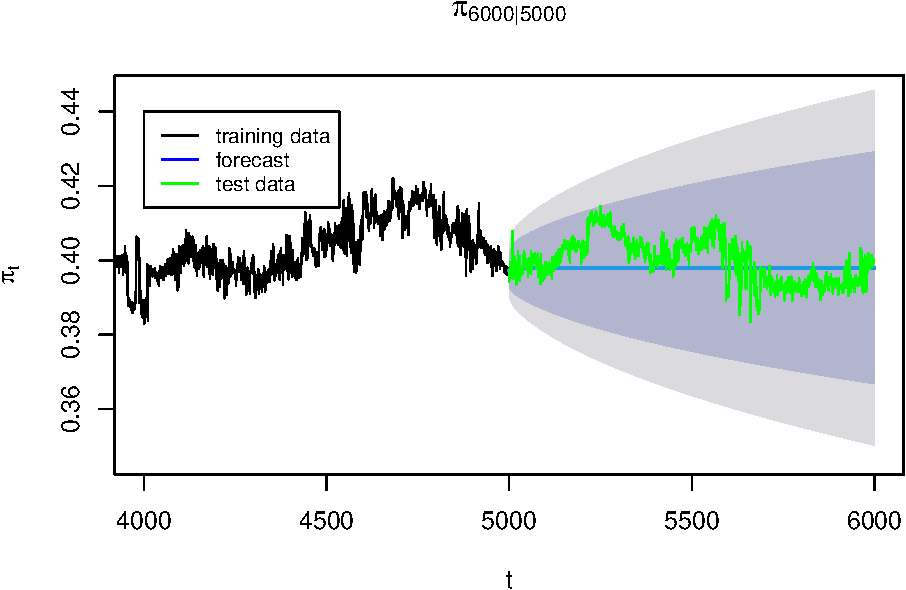
\includegraphics{paper_files/figure-latex/unnamed-chunk-16-1.pdf}
\caption{Forecasting the future with the training set and test sets superimposed.}
\label{fig:forecast}
\end{figure}

The held out \emph{test} data remains within the \(80\%\) prediction
interval for most of the time. All things considered, this seems like a
reasonable forecast. However, due to what we believe may be a
\emph{model} misspecification, we think the prediction intervals are too
wide and we have reason to believe that, in the long run, \(\{\pi_t\}\)
will decrease in variance and hover around some asymptotic limit. We
explore this more in the next section.

\hypertarget{incorporating-information}{%
\subsection{\texorpdfstring{Incorporating \emph{a priori}
information}{Incorporating  information}}\label{incorporating-information}}

We have \emph{a priori} knowledge that we wish to incorporate into the
model. Assuming the plaintext distribution \(\{x_t\}\) is static and the
algorithm that converts plaintext to ciphers is fixed, we observe the
following:

\begin{enumerate}
\item The accuracy of the adversary, $\pi_t$, is a measure between $0$ and $1$.
\item Under ideal conditions, acquiring more knowledge by observing a larger
sample is not expected to harm the adversary's accuracy $\pi_t$, in which case
the expectation $\pi_t$ would be a monotonically increasing function that has
an asymptotic limit $c \leq 1$.
\end{enumerate}

Of course, at different points in time the adversary's accuracy may
change due to, say, the presence of significant unaccounted covariates.

An ideal model for these axioms may be something like the Gompertz model
or even a \emph{scaled}, \emph{relocated}, and \emph{shifted} cumulative
distribution function (cdf). However, for the sake of model simplicity,
we assume a logarithmic form, which allows us to use linear regression.
It does not have an asymptotic limit, but we hypothesize that it is a
reasonable approximation for most finite time-horizons of interest.

Thus, we suppose the time series \(\{\pi_t\}\) has the functional form
\[
  \pi_t = \beta_0 + \beta_1 \log t.
\]

Instead of i.i.d. ``errors'' (deviations from the mean), we have reason
to believe the errors are correlated. We choose to model these errors in
the \(\arima\) family, such that \(\{\Pi_t\}\) is a random process of
the form \[
  \Pi_t = \beta_0 + \beta_1 \log t + \eta_t
\] where \[
  \eta_t \sim \arima(p,d,q).
\]

Actually, this is not quite true, since according to \cite{rob_arimax},
``The presence of lagged values {[}\ldots{]} means that \(\beta_1\) can
only be interpreted conditional on the value of previous values of the
response variable, which is hardly intuitive.''

No matter, we press on and fit the model to the data, which yields the
sought after ARIMA regression errors for \(\{\eta_t\}\) and estimates
for the parameters.

\begin{verbatim}
## Regression with ARIMA(1,1,2) errors 
## 
## Coefficients:
##          ar1      ma1     ma2    xreg
##       0.8521  -1.4012  0.4355  0.0292
## s.e.  0.0234   0.0277  0.0211  0.0202
## 
## sigma^2 estimated as 6.828e-06:  log likelihood=45279.87
## AIC=-90549.73   AICc=-90549.73   BIC=-90513.68
\end{verbatim}

We have used the same model as before, except with the dynamic
regression on the logarithm of time \(t\). It turns out that, for the
dynamic regression, \(\arima(2,1,2)\) does better and enjoys tighter
prediction intervals as well, but it was not significantly better.

To assess whether the model results in uncorrelated residuals, we
insepect figure \ref{fig:res}.

\begin{figure}
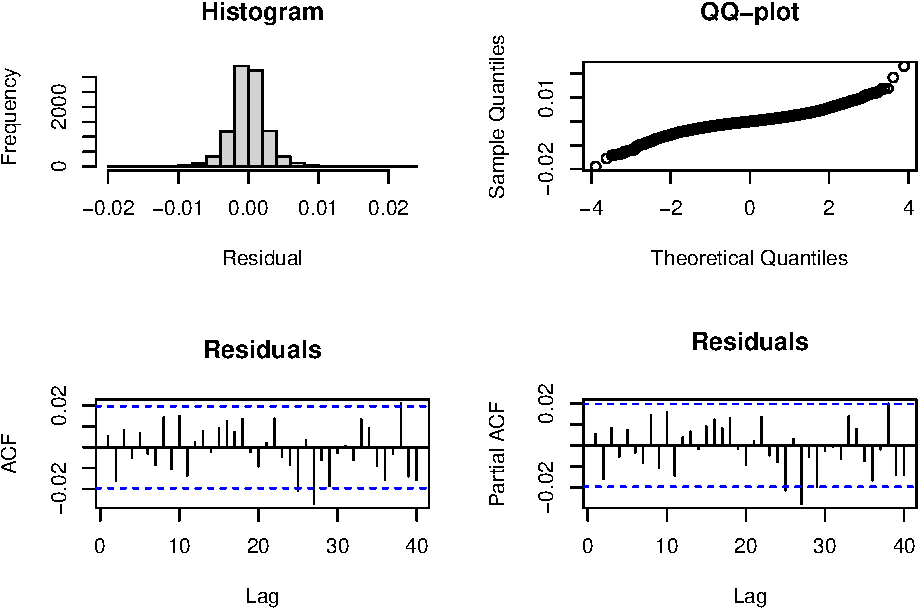
\includegraphics{paper_files/figure-latex/unnamed-chunk-18-1.pdf}
\caption{Plots to conduct stationary assessments}
\label{fig:res}
\end{figure}

The histogram looks symmetric about \(0\) but, again, the Q-Q suggests a
lack of normality in the residuals. However, the sample ACF and PACF
seem reasonable. We perform the Ljung-Box hypothesis (lag = 10) test on
the residuals of the model for a more objective measure of white noise.

\begin{verbatim}
## Box-Ljung test
## data:  reg_model$residuals
## X-squared = 10.279, df = 6, p-value = 0.1134
\end{verbatim}

At the \(5\%\) significance level, this model barely passes. We see that
\[
  \hat{\Pi}_t = 0.029 \log t + \eta_t
\] where \[
  \eta_t \sim \arima(5,1,1)
\] with the above specified estimated coefficients and \[
  e_t \sim \operatorname{WN}(\mu=0,\sigma=0.0026).
\]

We show a time series plot of the model with both the training set (in
black) and the test set (in green) superimposed onto it in figure \ref{fig:theory}.

\begin{figure}
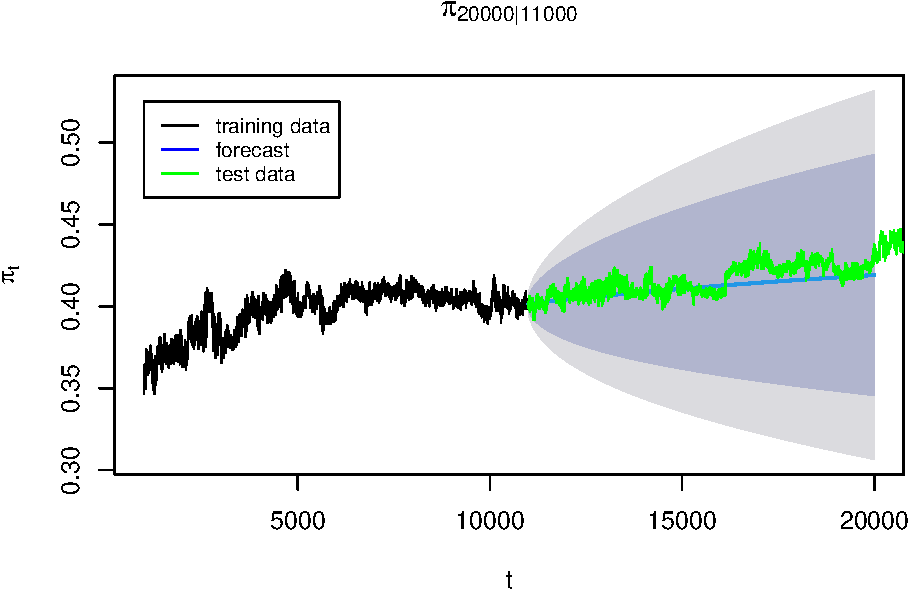
\includegraphics{paper_files/figure-latex/unnamed-chunk-20-1.pdf}
\caption{Forecast distribution of more appropriate theoretical model
of the time series.}
\label{fig:theory}
\end{figure}

We have forecasted much further into the future. The forecast seems
reasonable, as it follows the subtle positive non-linear trend.

When we compare it to the previous ARIMA model, we see that the subtle
positive trend is not captured by the model. We can address this
potential shortcoming by forcing the ARIMA model to include the drift
term. When we do this, we get the following results.

\begin{verbatim}
##           ar1           ma1           ma2         drift 
##  8.472755e-01 -1.396547e+00  4.324823e-01  4.695287e-06
\end{verbatim}

We see that the drift term is a positive value near \(0\), but over a
sufficiently long period of time it adds up, as demonstrated by the
figure \ref{fig:drift}.

\begin{figure}
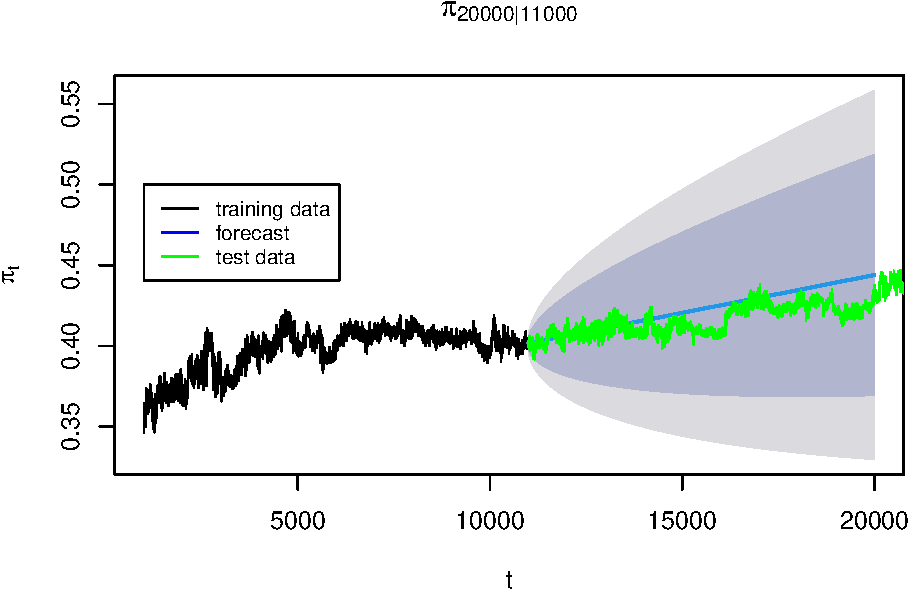
\includegraphics{paper_files/figure-latex/unnamed-chunk-22-1.pdf}
\caption{Forecast dsitribution of the ARIMA model with drifting.}
\label{fig:drift}
\end{figure}


The \(\arima\) model with drift adds a linear element to the
autoregression, which theoretically is not appropriate.

\hypertarget{future-work-dynamic-regression-on-co-variates}{%
\section{Future work: dynamic regression on
co-variates}\label{future-work-dynamic-regression-on-co-variates}}

\label{sec:future} In our time series analysis, the forecasting model
only used lagged values of the confidentiality measure to forecast
future values and we made no attempt to discover any other co-variates.
Therefore, it extrapolated trends but ignored any other information such
as \emph{side-channel} information that may help or hinder the
adversary's efforts to decode the ciphers.

At a time \(t'\), the adversary may learn something about the system
other than observing the time series of ciphers, \(\{C_t\}\). This
information may be incorporated into the time series model through an
autoregression that has predictor variables other than just lagged
components of the measure on the adversary's accuracy, \(\{\pi_t\}\).
The estimated paramters of the dynamic autoregressive model may also be
used to explain the effect such predictor variables have on
confidentiality.

A potentially interesting model is given by the data \[
  (t, \pi_t, I_t)
\] where \(t\) denotes time index, \(\pi_t\) denotes the adversary's
accuracy at time \(t\), and \(I_t\) denotes the \emph{information}
measure of the \(t\)-th observation, defined as \[
  I_t = \log_2 \frac{1}{\Pr(\operatorname{g}(c_{t'}))}.
\]

Observe that lagged components of \(I_t\) may be used to make the
regression a function of entropy \(H_t\) as well.

When the entropy is reduced or an informative observation comes in, this
may have a larger impact on the time series \(\{\pi_t\}\) and ideally we
would incorporate this effect into the model.

The information gain does not necessarily need to be related to any of
the time series previously mentioned, either. For instance, suppose the
adversary, through side-channel information, acquires the knowledge that
a certain cipher \(c'\) maps to some smaller subset
\(\set{W} \subset \set{X}\). This also may be modeled as an information
gain or entropy reduction, since the distribution of ciphers \(\{c_t\}\)
has less entropy given this information.

\hypertarget{conclusion}{%
\section{Conclusion}\label{conclusion}}
The statician George Box once wrote, ``All models are wrong, some are useful.''
If we include \emph{drifting} in the ARIMA model, it eventually predicts
impossible futures.
More to the point, it is not a good match for the theoretical model, as its
bias is a function of time $t$.

The logarithmic model performs better in this regard, as it takes an
inordinately long time (1,531,520,000,000,000 steps) to reach impossible
values, although the prediction interval obtains it much more quickly.
In addition, it more closely matches the features of the theoretical
underlying distribution.

That said, there is still a lot to be said of the $\arima()1,1,2)$ model,
given its simplicity.
The adversary takes a very long time before it starts to seem like the
simple model may be negatively biased.

Recall that if we specify that $\pi^* = 0.44$ is the minimum confidentiality
we wish to maintain, a reasonable policy may be to use the latest
observation to forecast the future to estimate where $\pi_t = \pi^*$,
which is given by
$$
    \hat{T}^* = \argmin_{T} \pi_{T\,|\,11000} > \pi^*.
$$

\begin{figure}
    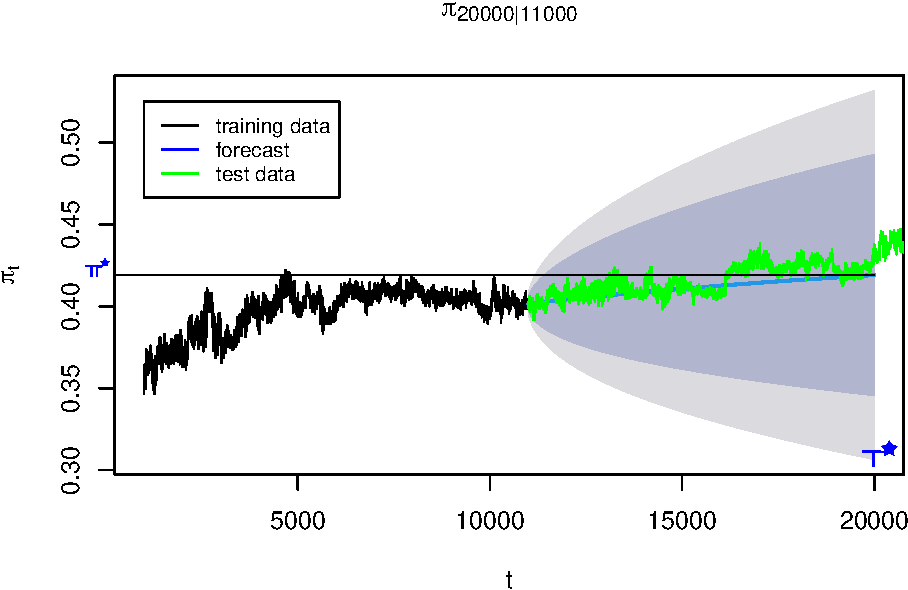
\includegraphics{Tstar.pdf}
    \caption{$\pi^*$ vs $T^*$.}
    \label{fig:tstar}%      only if needed  
\end{figure}

Inspecting figure \ref{fig:tstar}, we see that $\hat{T}^* \approx 20000$.
That is, to maintain $\pi^* > 0.44$, a password reset should occur
before $T^* \approx 20000$.

Interestingly, the prediction intervals are far less forgiving and
if we used those as a pessimistic estimator of $T^*$, we would
nearly instantaneouls need to do a password reset.

To be a useful measure, it would seem that the uncertainty should be
lower.
Possibly, as we discuss in section \ref{sec:future}, we could
incorporate other covariates that help reduce the uncertainty.
Or, perhaps we need to impose a more realistic dynamic trend.
After all, the logarithm is not a particularly good fit for the
data either, it is simply potentially better than the other
alternatives.



\bibliography{refs.bib}
\bibliographystyle{plainurl}

\end{document}
